\documentclass[12pt]{article}
\linespread{1.3}
\usepackage{scrextend}
\usepackage{hyperref}
\usepackage{enumitem}
%\usepackage{enumerate}
\usepackage{changepage,lipsum,titlesec, longtable}
\usepackage{cite}
\usepackage{comment, xcolor}
\usepackage[pdftex]{graphicx}
  \graphicspath{{images/}, {images/stat/}}
  \DeclareGraphicsExtensions{.pdf,.jpeg,.png, .jpg}
\usepackage[cmex10]{amsmath}
\usepackage{array} 
\usepackage{subfigure} 
\usepackage{placeins} 
\usepackage{amsfonts}
\usepackage{pifont}% http://ctan.org/pkg/pifont
\usepackage{minted}
\usepackage{bbm}

\newcommand{\cmark}{\ding{51}}%
\newcommand{\xmark}{\ding{55}}%
\newcommand{\grey}[1]{\textcolor{black!30}{#1}}
\newcommand{\red}[1]{\textcolor{red!50}{#1}}
\newcommand{\fref}[1]{Figure~\ref{#1}}
\newcommand{\tref}[1]{Table~\ref{#1}}
\newcommand{\eref}[1]{Equation~\ref{#1}}

\oddsidemargin0cm
\topmargin-2cm %I recommend adding these three lines to increase the
\textwidth16.5cm %amount of usable space on the page (and save trees)
\textheight23.5cm

\makeatletter
\renewcommand\paragraph{\@startsection{paragraph}{4}{\z@}%
            {-2.5ex\@plus -1ex \@minus -.25ex}%
            {1.25ex \@plus .25ex}%
            {\normalfont\normalsize\bfseries}}
\makeatother
\setcounter{secnumdepth}{4} % how many sectioning levels to assign numbers to
\setcounter{tocdepth}{4}    % how many sectioning levels to show in ToC

\begin{document}
\title{Regression based energy model and building energy saving calculation: analyzing the effect of temperature variable representation, and plan of next step}
\maketitle
\tableofcontents
\newpage
% \begin{verbatim}
% occupied vs non-occupied: clustering?, time series analysis?
% boosting simple linear regression?
% pre-processing? and noise removal?
% \end{verbatim}
\section{Goal statement}
The broad goal of the study is to build a better (more accurate, or
more interpretable, or both) building energy baseline model.  The
result will be useful in the application of building load / demand /
consumption forcasting~\cite{dong2005applying, solomon2011forecasting,
  Yu20101637, mocanu2016deep, hammarsten1987critical}, calculation of
energy savings from energy conservation retrofits~\cite{haberl1994bin,
  edition2013ashrae, kissock2008methodology, kissock2003,
  fels1986prism}, evaluating building energy
performance~\cite{abushakra1997inverse}, building parameter
estimation~\cite{hammarsten1987critical}, energy end use
disaggregation~\cite{leanEng, fels1986prism, wytock2013contextually},
assist the ``identification of energy saving opportunities and
recommend the types of energy efficiency measures''~\cite{leanEng}.

The common input variable to the model include:
\begin{itemize}
\item Environmental variable
  \begin{itemize}
  \item Temperature (measured, average, or categorical): 
    \begin{itemize}
    \item outdoor air temperature
      \begin{itemize}
      \item as numerical: mean~\cite{haberl1994bin,
          hammarsten1987critical, kissock2008methodology,
          dong2005applying, leanEng},
        degree-day~\cite{reddy1997baselining, fels1986prism,
          pmWeather}, Radio Basis Function Kernel
        (RBFs)~\cite{wytock2013contextually},
        exact~\cite{mackay1996bayesian, Zhang2015177, cao2003support}
      \item as categorical variables~\cite{Yu20101637}
      \end{itemize}
    \item indoor air temperature~\cite{hammarsten1987critical}
    \end{itemize}
  \item Humidity
    \begin{itemize}
    \item relative humidity (RH)~\cite{dong2005applying}
    \item dew point temperature~\cite{cao2003support}
    \item exponential smoothing applied to humidity with time constant of 24h~\cite{brown2012kernel}
    \end{itemize}
  \item Solar: 
    \begin{itemize}
    \item solar radiation ($W / m^2$)~\cite{hammarsten1987critical, dong2005applying, flouquet1992local}
    \item solar flux~\cite{mackay1996bayesian}
    \item solar aperture ($m^2$)~\cite{hammarsten1987critical}, different in different time of year
    \item solar gains ($Q_S = SI, \text{unit: } W$)~\cite{hammarsten1987critical}
    \end{itemize}
  \item Wind 
    \begin{itemize}
    \item speed~\cite{mackay1996bayesian}
    \item velocity~\cite{brown2012kernel}
    \end{itemize}
  \end{itemize}
\item Occupancy
  \begin{itemize}
  \item Number of occupants~\cite{Yu20101637}
  \item Operation schedules~\cite{reddy1997baselining}
  \item Occupancy ratio (ratio of occupied vs non-occupied days)~\cite{rabl1992energy}
  \end{itemize}
\item Industry type
\item Building construction
  \begin{itemize}
  \item Detached vs apartment, categorical~\cite{Yu20101637}
  \item Construction material: wooden vs non-wooden~\cite{Yu20101637}
  \end{itemize}
\item Time
  \begin{itemize}
  \item day type (every-day, weekday, weedend)~\cite{haberl1994bin}
  \item hour of day (~\cite{haberl1994bin, wytock2013contextually},
    ~\cite{granderson2014evaluation} mean-week and
    day-time-temperature regression model)
  \item day of week (~\cite{granderson2014evaluation} mean-week, 
    day-time-temperature, and LBNL regression model)
  \item time lag ($k$), the number of previous readings to include in the model~\cite{hammarsten1987critical}
  \item unit circle representation of time of day, week, month, and year~\cite{brown2012kernel}
  \end{itemize}
\item Energy
  \begin{itemize}
  \item power ($W$, it's an auto-regressive component: use energy to
    predict energy)
    ~\cite{hammarsten1987critical, case2012saving}(\cite{mocanu2016deep} has some
    experiment about prediction of different time horizon using
    different time resolution)
  \item fuel type: Electric vs non-electric ~\cite{Yu20101637}
  \item Lighting and receptacle use~\cite{kissock1994modeling}
  \end{itemize}
\item Floor area~\cite{Yu20101637}
\item Building dynamics
  \begin{itemize}
  \item Heat loss coefficient ($W / m^2K$)~\cite{Yu20101637}
  \item Equivalent leakage area ($cm^2 / m^2$)~\cite{Yu20101637}
  \end{itemize}
\item Retrofit type / time
  \begin{itemize}
  \item pre-retrofit period~\cite{kissock2008methodology}
  \end{itemize}
\end{itemize}

The common output could be whole building energy such as whole building
electricity~\cite{haberl1994bin} or gas, or single end use such as air
handler unit (AHU) electricity~\cite{haberl1994bin}, chilled water
energy~\cite{haberl1994bin}, chiller energy
~\cite{abushakra1997inverse}, condenser
energy~\cite{abushakra1997inverse}, hot water
energy~\cite{haberl1994bin, abushakra1997inverse}, AC-electric,
appliance-electric, base-electric~\cite{wytock2013contextually}.

% For personal development, it is also a good practice of statistics /
% machine learning techniques (topics involved in this field include
% linear regression, SVM, Kernel Regression, regularization, clustering,
% PCA, neuron network (including deep learning).

In literature, the topic is commonly referred to as: whole building or
building baseline models~\cite{granderson2014evaluation,
  reddy1997baselining, kissock2008methodology, dong2005applying,
  Zhang2015177}, weather-adjusted index of
consumption~\cite{fels1986prism}, energy signature
model~\cite{rabl1992energy, hammarsten1987critical}, inverse (energy)
model~\cite{kissock2003, abushakra1997inverse, Zhang2015177},
data-driven (energy) models~\cite{Zhang2015177}, energy prediction
model~\cite{mocanu2016deep, Yu20101637, dong2005applying}.

\section{Scope}
The document presents the results of analyzing the influence of the
temperature representation on model prediction accuracy.

In previous works, the most common representation of temperature used are:
\begin{itemize}
\item raw temperature
\item average temperature
\begin{equation}
  \label{eq:ave_temp}
  \text{average temperature} = E[T_i]
\end{equation}
\item degree-day
\begin{equation}
  \label{eq:cool-degree-day}
  \text{cooling degree-day} = \sum_{i = 1}^n(T_i - T_{base})\mathbbm{1}(T_i > T_{base})
\end{equation}
\begin{equation}
  \label{eq:heat-degree-day}
  \text{heating degree-day} = \sum_{i = 1}^n(T_{base} - T_i)\mathbbm{1}(T_i < T_{base})
\end{equation}
\item smoothed with exponential weighting function~\cite{brown2012kernel, expSmoothWiki2016}
  \begin{equation}
    \label{eq:expsmooth}
    s_0 = x_0; s_t = \alpha x_t + (1 - \alpha)s_{t - 1}
  \end{equation}
  \begin{equation}
    \label{eq:timeconst}
    \alpha = 1 - \exp(-\frac{\Delta T}{\tau})
  \end{equation}
  \cite{expSmoothWiki2016}
\item radio basis function~\cite{wytock2013contextually}: defined to
  be some function $\phi$ such that
  $\phi(x) = \phi(\left\|x\right\|)$~\cite{rbfWiki2016}, it's a
  non-linearly transformed degree-day representation to approximate /
  smooth the environment (temperature) input
  \begin{equation}
    \label{eq:rbf_functionapprox}
    y(\mathbf{x}) = \sum_{i = 1}^N w_i \phi(\left\|\mathbf{x} - \mathbf{x_i}\right\|)
  \end{equation}~\cite{rbfWiki2016}
\end{itemize}

It is very common that the time resolution of the temperature data and
the energy data is different: the common time step for temperature is
usually hourly, while the energy data could be sub-hourly as in the
case of smart meter measured values, or monthly in the case of utility
bills. There is a tendency to unify the two variables into the same
time resolution: when only monthly utility bills are available, the
temperature is usually aggregated into a single value for each month,
the average temperature, or the degree day.

However, such aggregation might lose some detailed information of the
temperature changes, thus could affect the prediction accuracy of a
model. The average monthly temperature approach does not record the
temperature fluctuation, so a climate with very hot day and very cold
night could have the same average temperature as the one with very
stable temperature throughout the whole months, but the former would
use a lot more heating and cooling energy comparing to the latter. The
degree-day reflects more about the cooling and heating load, but the
choice of $T_{base}$ could affect the value of the degree-day. One way
to choose a base temperature is to fit a linear regression model for a
range of candidate $T_{base}$ and choose the fit with the highest
$R^2$. After choosing this single $T_{base}$, we assumed that the
heating is only relevant to the temperature above that base (for
cooling) or below that base for heating. Whether there's such a hard
turning point is not certain.

Based on the previous observations, two general thoughts of how to
improve the models using either aggregation method is: 1) can we
remove the aggregation completely? 2) can we use some smarter
aggregation method?

Thus the following approaches are proposed:
\begin{itemize}
\item No aggregation: Use the vector of hourly temperature for each
  month as the independent variable, with regularization.
\begin{figure}[h!]
  \centering
  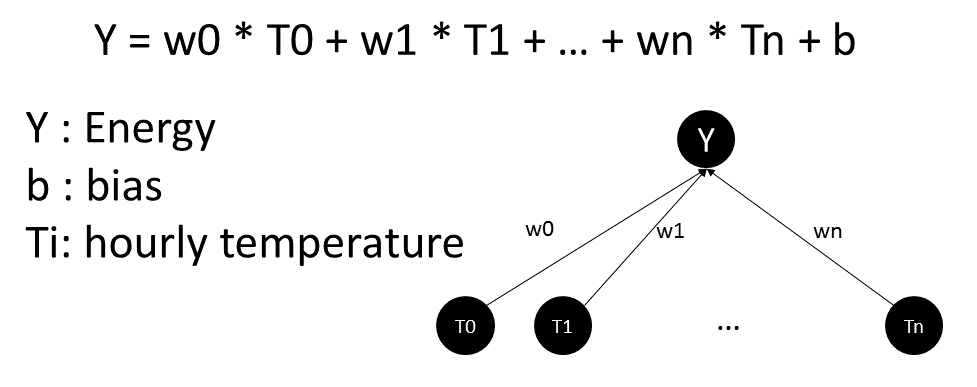
\includegraphics[width=0.7\textwidth]{images/Slide16.PNG}
  \caption{method 1 diagram}
\end{figure}
\item Smarter aggregation
\begin{figure}[h!]
  \centering
  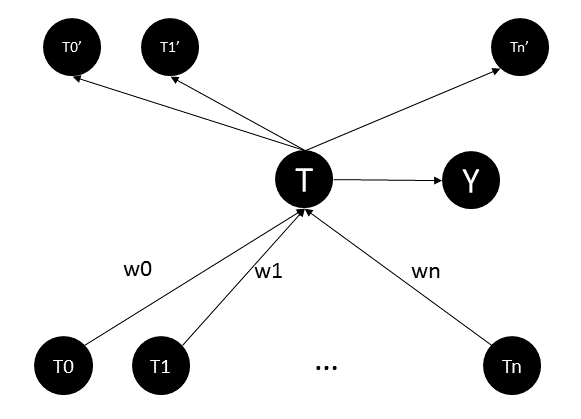
\includegraphics[width=0.5\textwidth]{images/Slide17.PNG}
  \label{fig:pcafig}
  \caption{method 1 diagram}
\end{figure}
\FloatBarrier
    \begin{itemize}
    \item Pre-process hourly temperature with PCA
    and use the projected input as the independent variable.
  \item Learn an auto-encoder of the hourly temperature to get some
    lower dimension hidden representation and use the lower
    dimensional representation as the independent variable.
  \item Keep many degree-day variables in the model, with a set of
    different bases, and regularize with fused
    lasso~\cite{tibshirani2005sparsity}
    \end{itemize}
\end{itemize}
These methods are to be compared with two baseline methods: The
piecewise regression model with monthly mean temperature as the
independent variable; the best-fit (highest $R^2$) degree-day model.
\section{Process}
% The following four methods will be implemented:
% \begin{itemize}
% \item Use hourly temperature with ridge term.
% \item Use the first few Principal Components (that preserves 95\% of the variance) of the hourly temperature with month duration.
% \item Learn a auto-encoder that contains a non-linear activation function.
% \item Use fused lasso with all degree days as the regression term.
% \end{itemize}
The data is randomly split into a train-development set, and a test
set. This is done with the
\texttt{sklearn.model\_selection.train\_test\_split} For the ridge
regression approach, the train-development set is used to tune the
ridge parameter with cross validation and also learn model, the test
set is used to report the performance.

Before performing regression, the $X$ should be standardized by
$x_i' = (x_i - E[X])/\sigma_X$, and $Y$ should be centered by
$y_i' = y_i - E[Y]$(??)~\cite{ridgeRegTib2006}

The following result is based on the experiment with the building \href{http://128.2.109.159:8080/GSA/interval/trend/OR0033PE_gas.html}{``OR0033PE''}.
\begin{figure}[h]
  \centering
  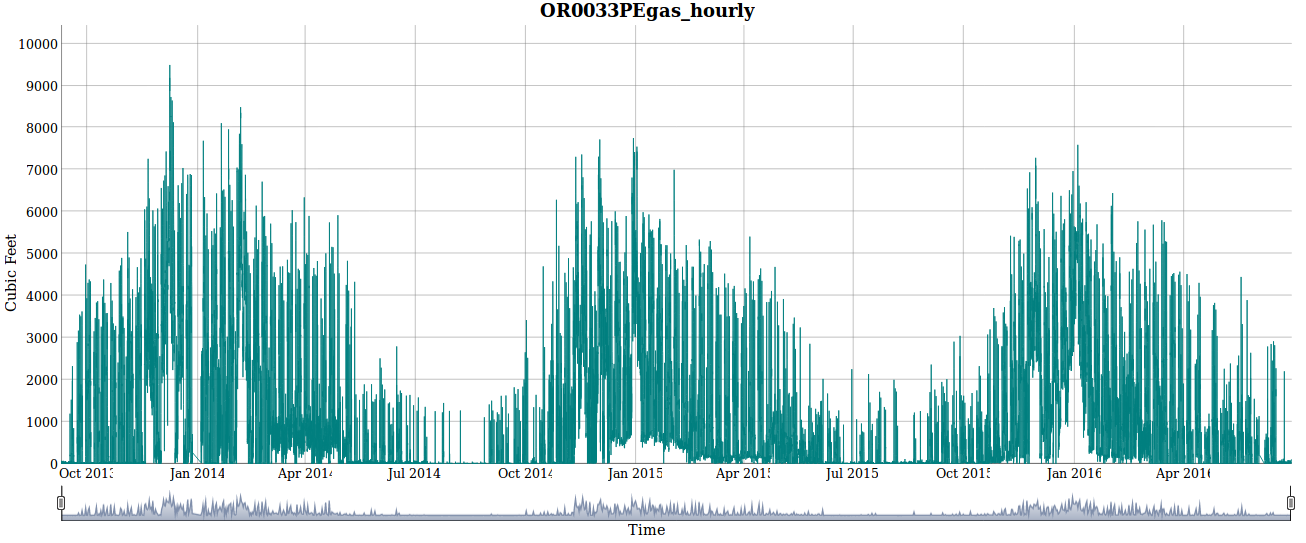
\includegraphics[width=0.7\textwidth]{images/or0033peTrend.png}
\end{figure}
\subsection{Baseline method: piecewise linear regression with average month temperature}
MSE: 2.07631642389
\subsection{Proposed method 1: Hourly temperature with ridge term}
Given the data $\mathcal{D} = \{(\mathbf{x^{(i)}}, y^{(i)})\}^n$,
where $\mathbf{x^{(i)}} \in \mathbb{R}^{T_i}$ is the hourly
temperature of the i-th month, $T^{(i)}$ is the number of hours in the
i-th month. For simplicity, $T^{(i)}$ is fixed to
$720 = 24 \times 30$. $y^{(i)} \in \mathbb{R}$ is the monthly whole
building electricity or gas consumption.

The form of the regression mode is
\begin{equation}
  \label{eq:regression}
  \hat{y_i} = \mathbf{\theta}^T \cdot \mathbf{x^{(i)}}
\end{equation}
Note, since the data is pre-centered, there's no bias term in the
model.

The model is learned by minimizing the loss function \eref{eq:ridge}.
\begin{equation}
  \label{eq:ridge}
  J(\mathbf{\theta}) = \frac{1}{2}(\mathbf{\theta}^T\mathbf{x^{(i)}} - y^{(i)})^2 + \lambda \left\|\theta\right\|^2
\end{equation}
$\lambda$ is the ridge parameter that controls the amount of
regularization, it is tuned in the train-development set with
cross-validation. \texttt{sklearn.linear\_model.Ridge} is used for
compute the ridge regression.

Cross-validation is performed by first partitioning the
train-development data set into K folds. For the i-th fold, a model is
learned on the rest K - 1 folds ($\{K_j \mid j \neq i\}$), the error
is computed on the i-th fold. This process is repeated for K
times. The error metric is mean squared error, the overall error is
the average of the error of using the i-th fold as the test set. This
is done with \texttt{sklearn.model\_selection.cross\_val\_score}. In
this experiment, 5-fold cross validation is used.

In the ridge regression, the hyper parameter $\lambda$ needs to be
tuned with cross-validation. A plot of $\text{MSE} - \lambda$ is shown
in \fref{fig:cv_5_fold_ridge}
\begin{figure}[h!]
  \centering
  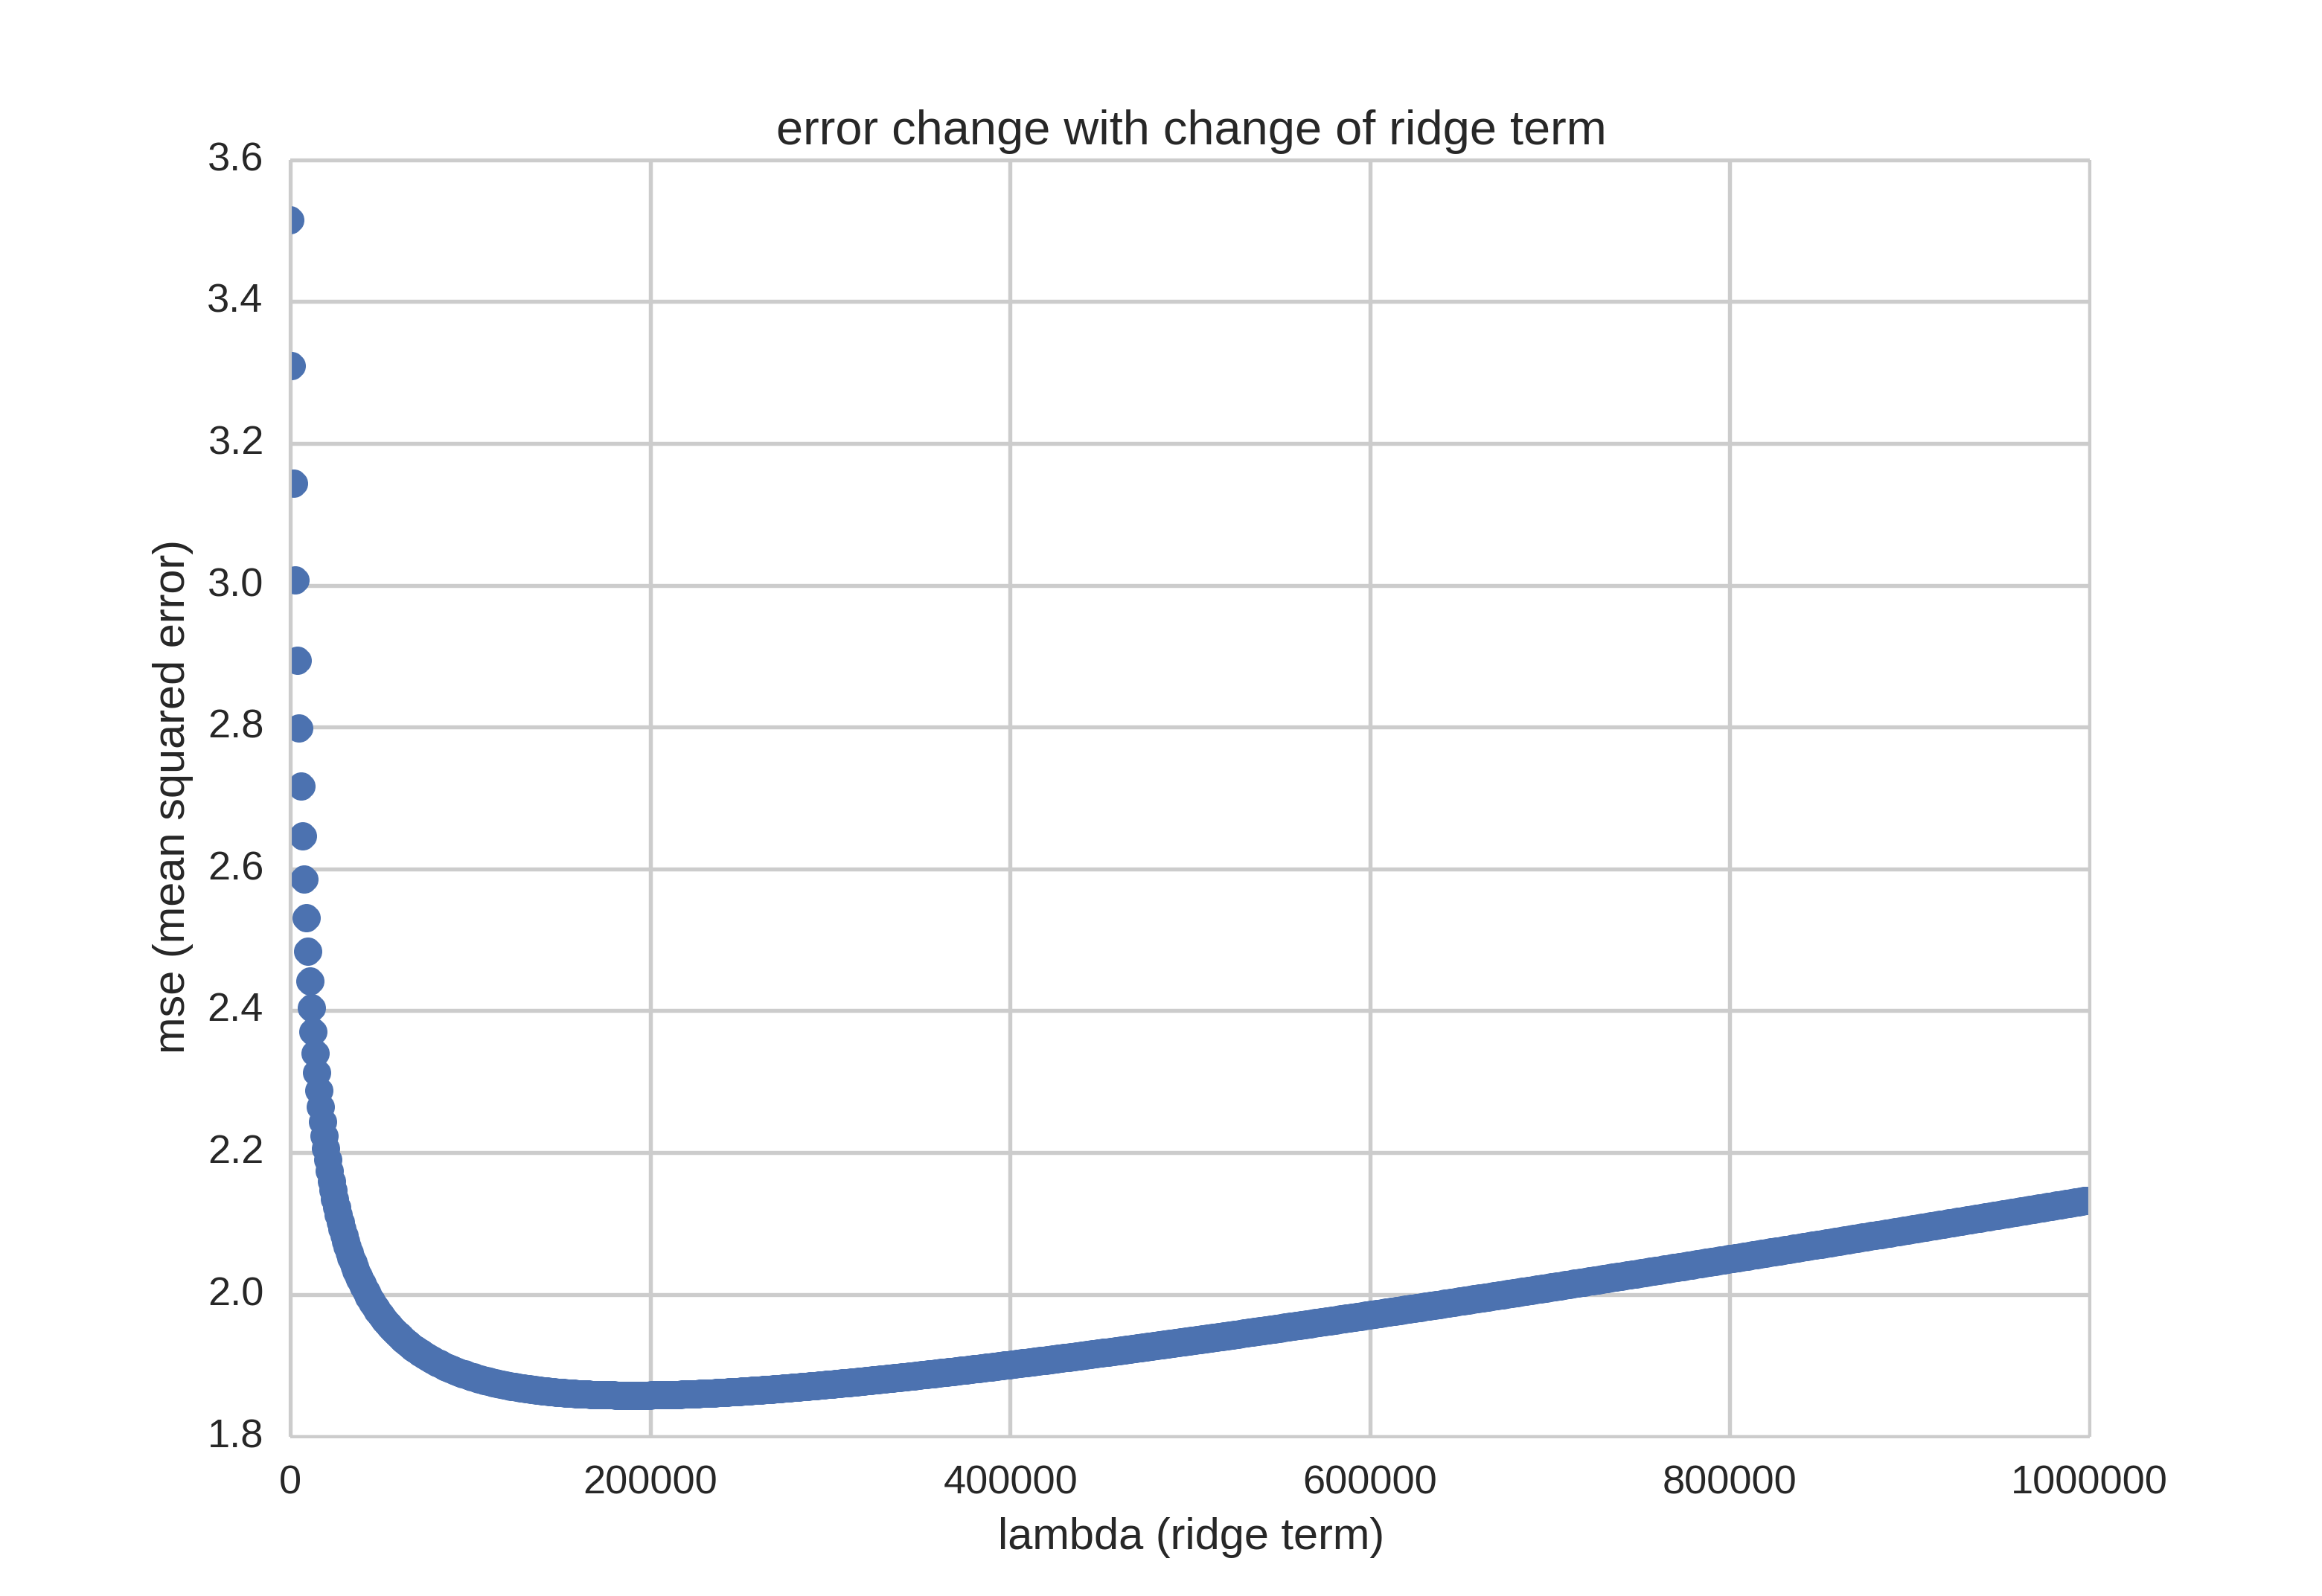
\includegraphics[width=0.6\textwidth]{images/cv_5_fold_ridge.png}
  \caption{MSE vs lambda plot}
  \label{fig:cv_5_fold_ridge}
\end{figure}
\FloatBarrier

From the plot, the $\lambda$ that gives the lowest error is around
190000. Using this optimal $\lambda$ to re-fit the model, we get the
model:
\begin{verbatim}
[ -1.55822925e-04  -1.42539701e-04  -1.09100028e-04  -4.06291050e-06
   8.84344833e-05   1.78332926e-04   2.68478265e-04   2.65000351e-04
   2.02735707e-04   1.39508922e-04   1.30677887e-04   1.08732504e-04
   8.07017042e-05   8.77490889e-05   1.00807169e-04   9.19141490e-05
   8.23187429e-05   7.24149582e-05   4.88254898e-05   7.27015617e-05
   1.01496385e-04   1.02519860e-04   9.03311707e-05   6.98651205e-05
   6.75534592e-05   1.24527082e-04   1.25621821e-04   1.27268793e-04
   ...
]
\end{verbatim}
\begin{figure}[h!]
  \centering
  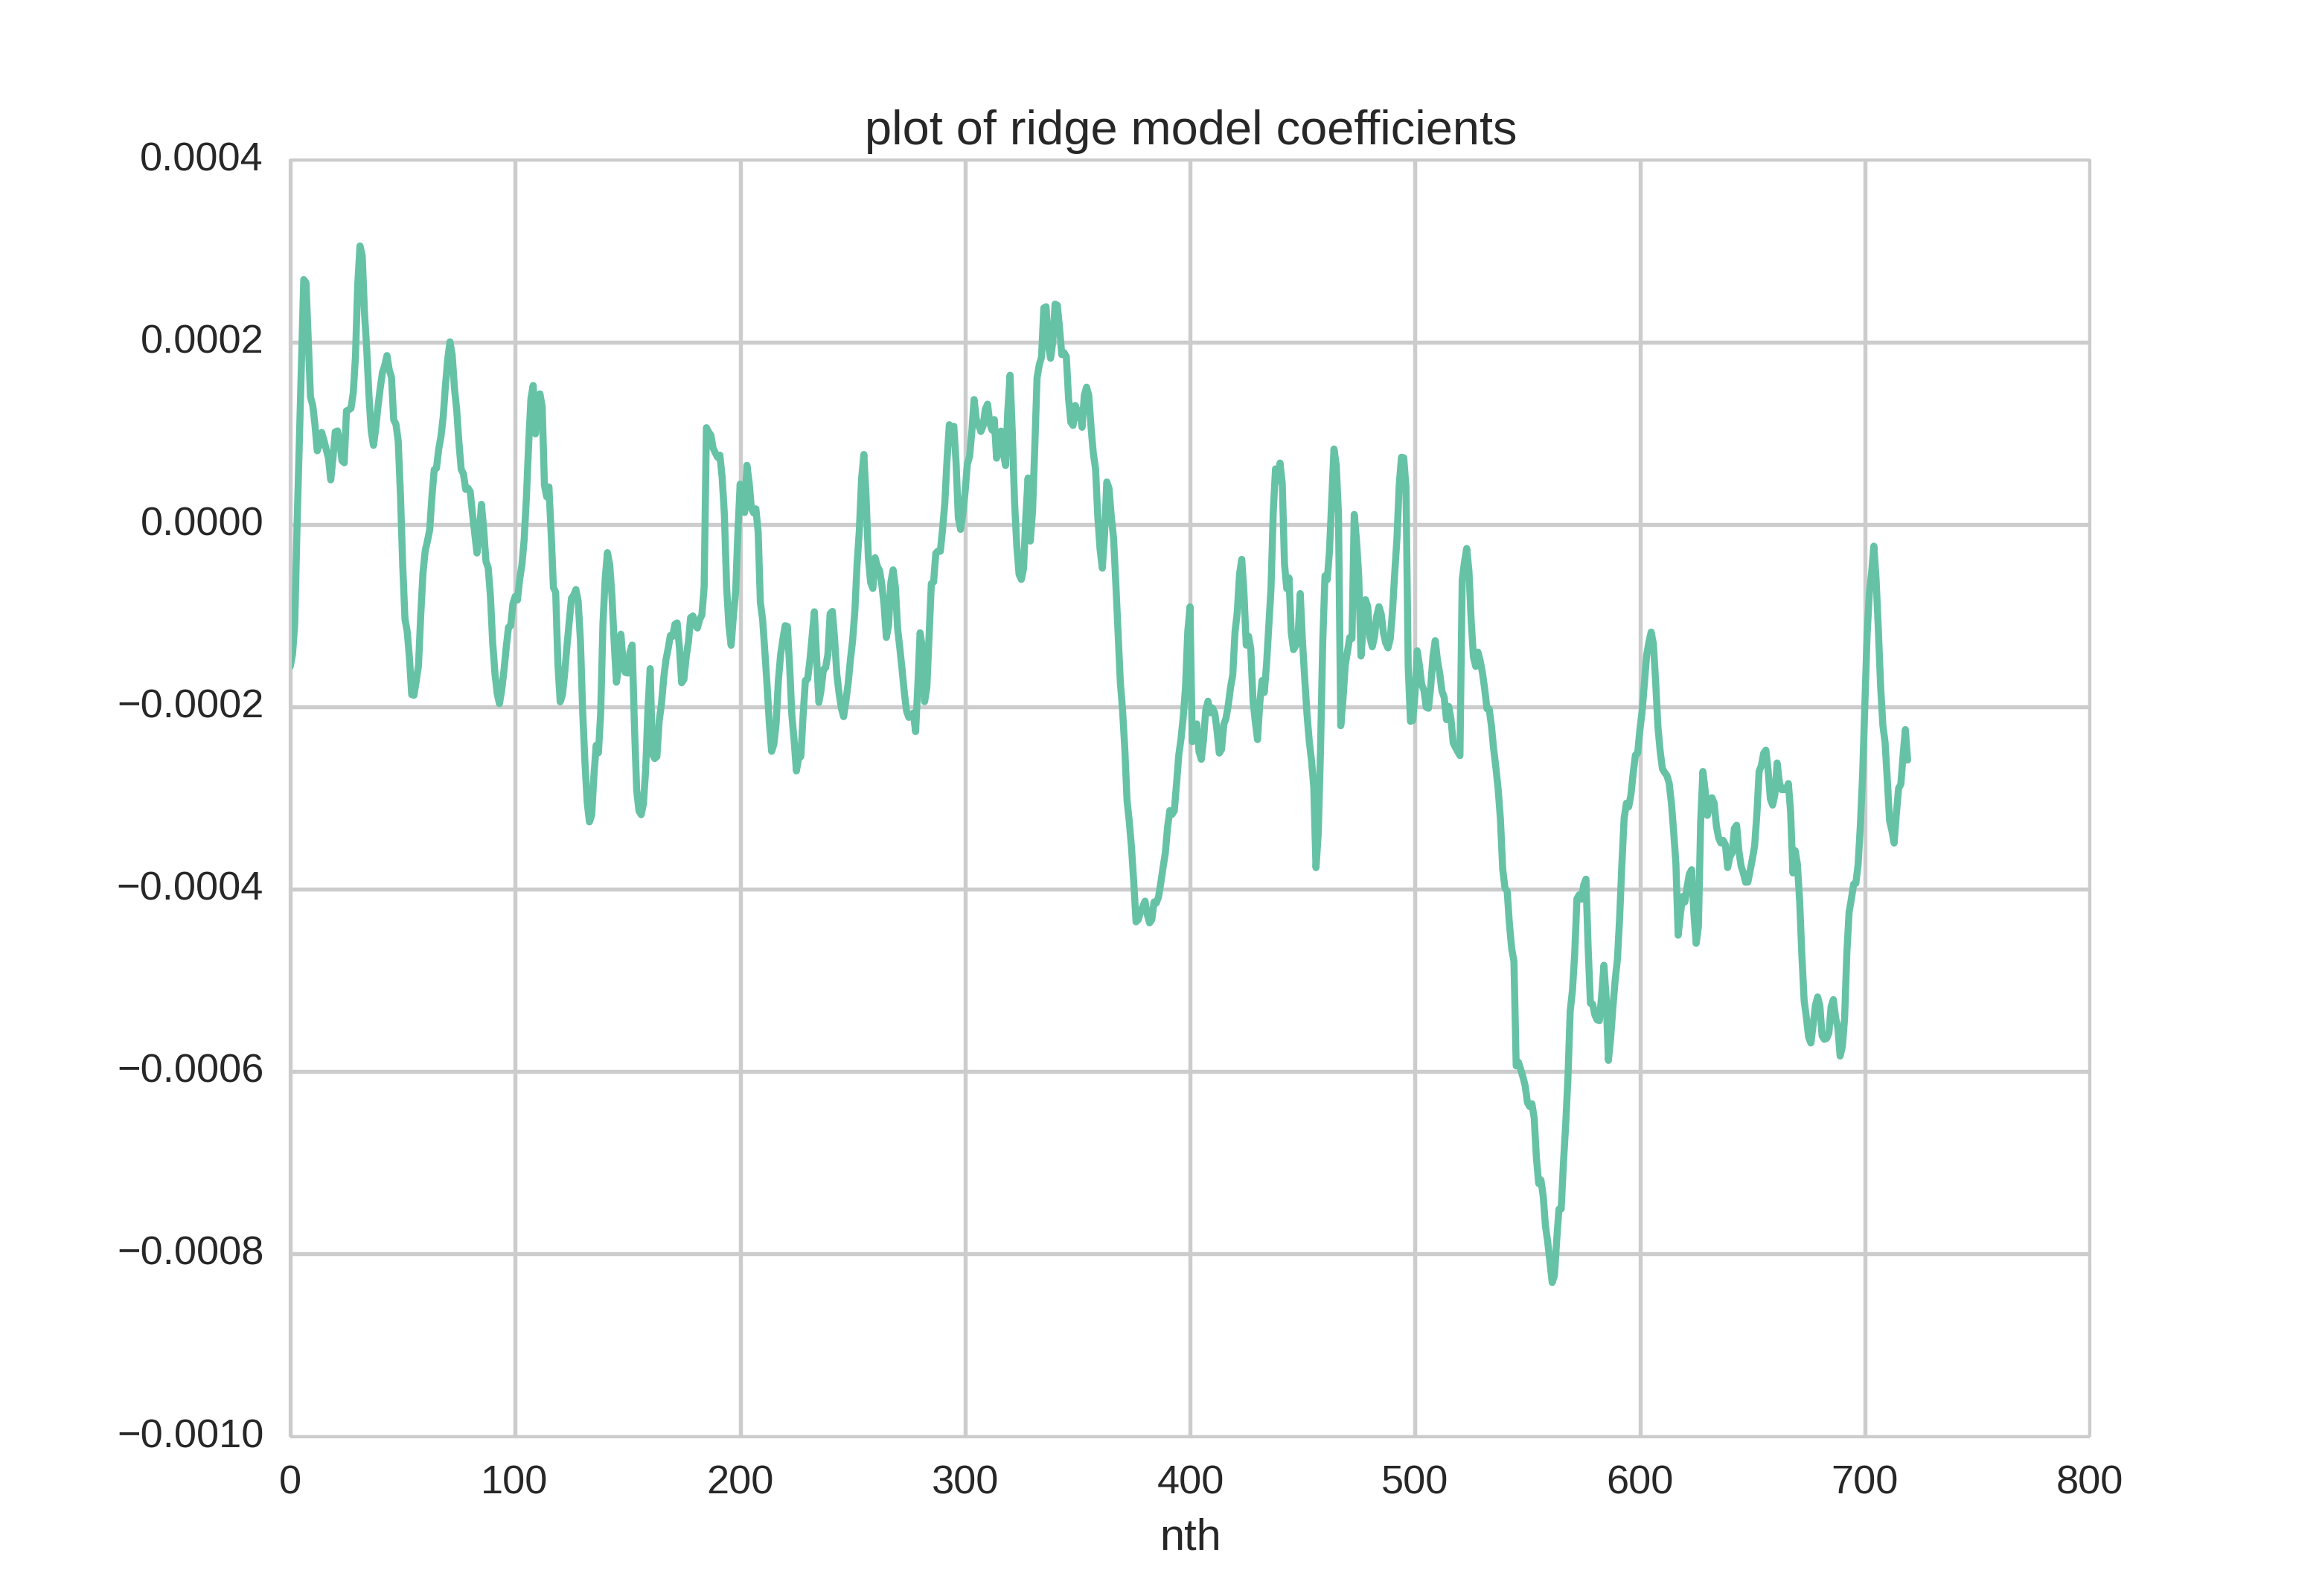
\includegraphics[width=0.6\textwidth]{images/param_ridge_opt.png}
  \caption{ridge regression parameter plot}
  \label{fig:param_ridge_opt}
\end{figure}
\FloatBarrier

From the plot of the parameters, the first two weeks seems to have
larger impact on the gas consumption. The MSE of the building is: 1.37049790455

Later development will use Baysian Optimization will be used to tune
the hyper parameters instead of the current grid search.
\subsection{Proposed method 2: PCA}
PCA regression ~\cite{pcrWiki2016} uses top PCs of the input data as
the independent variable for the regression. It is ``some kind of
regularized procedure''~\cite{pcrWiki2016}.
\subsubsection{result of analyzing weather station data}
By analyzing the data from 483 weather stations in the U.S. used in
the GSA project, the number of principal components with
re-construction error of 95 percent (top) 99 percent (bottom) is shown
in \fref{fig:num_pcs}

The input is a $720 \times m$ matrix $X$ (720 hours per month, for
simplicity), m is computed by \texttt{n / 720} (round down). Each
column in the matrix $X$ is a month worth of hourly temperature. The
data is re-centered by $X - \mu$, where $\mu$ is the average of $X$.

The principal components analysis is conducted with the eigen
decomposition of the covariance matrix, $XX^T$. The output include the
eigenvectors and the eigenvalues. The eigenvectors are the principal
components, and the ith eigenvalues are the variances accounted for by
the ith principal components. 
\begin{figure}[h!]
  \centering
  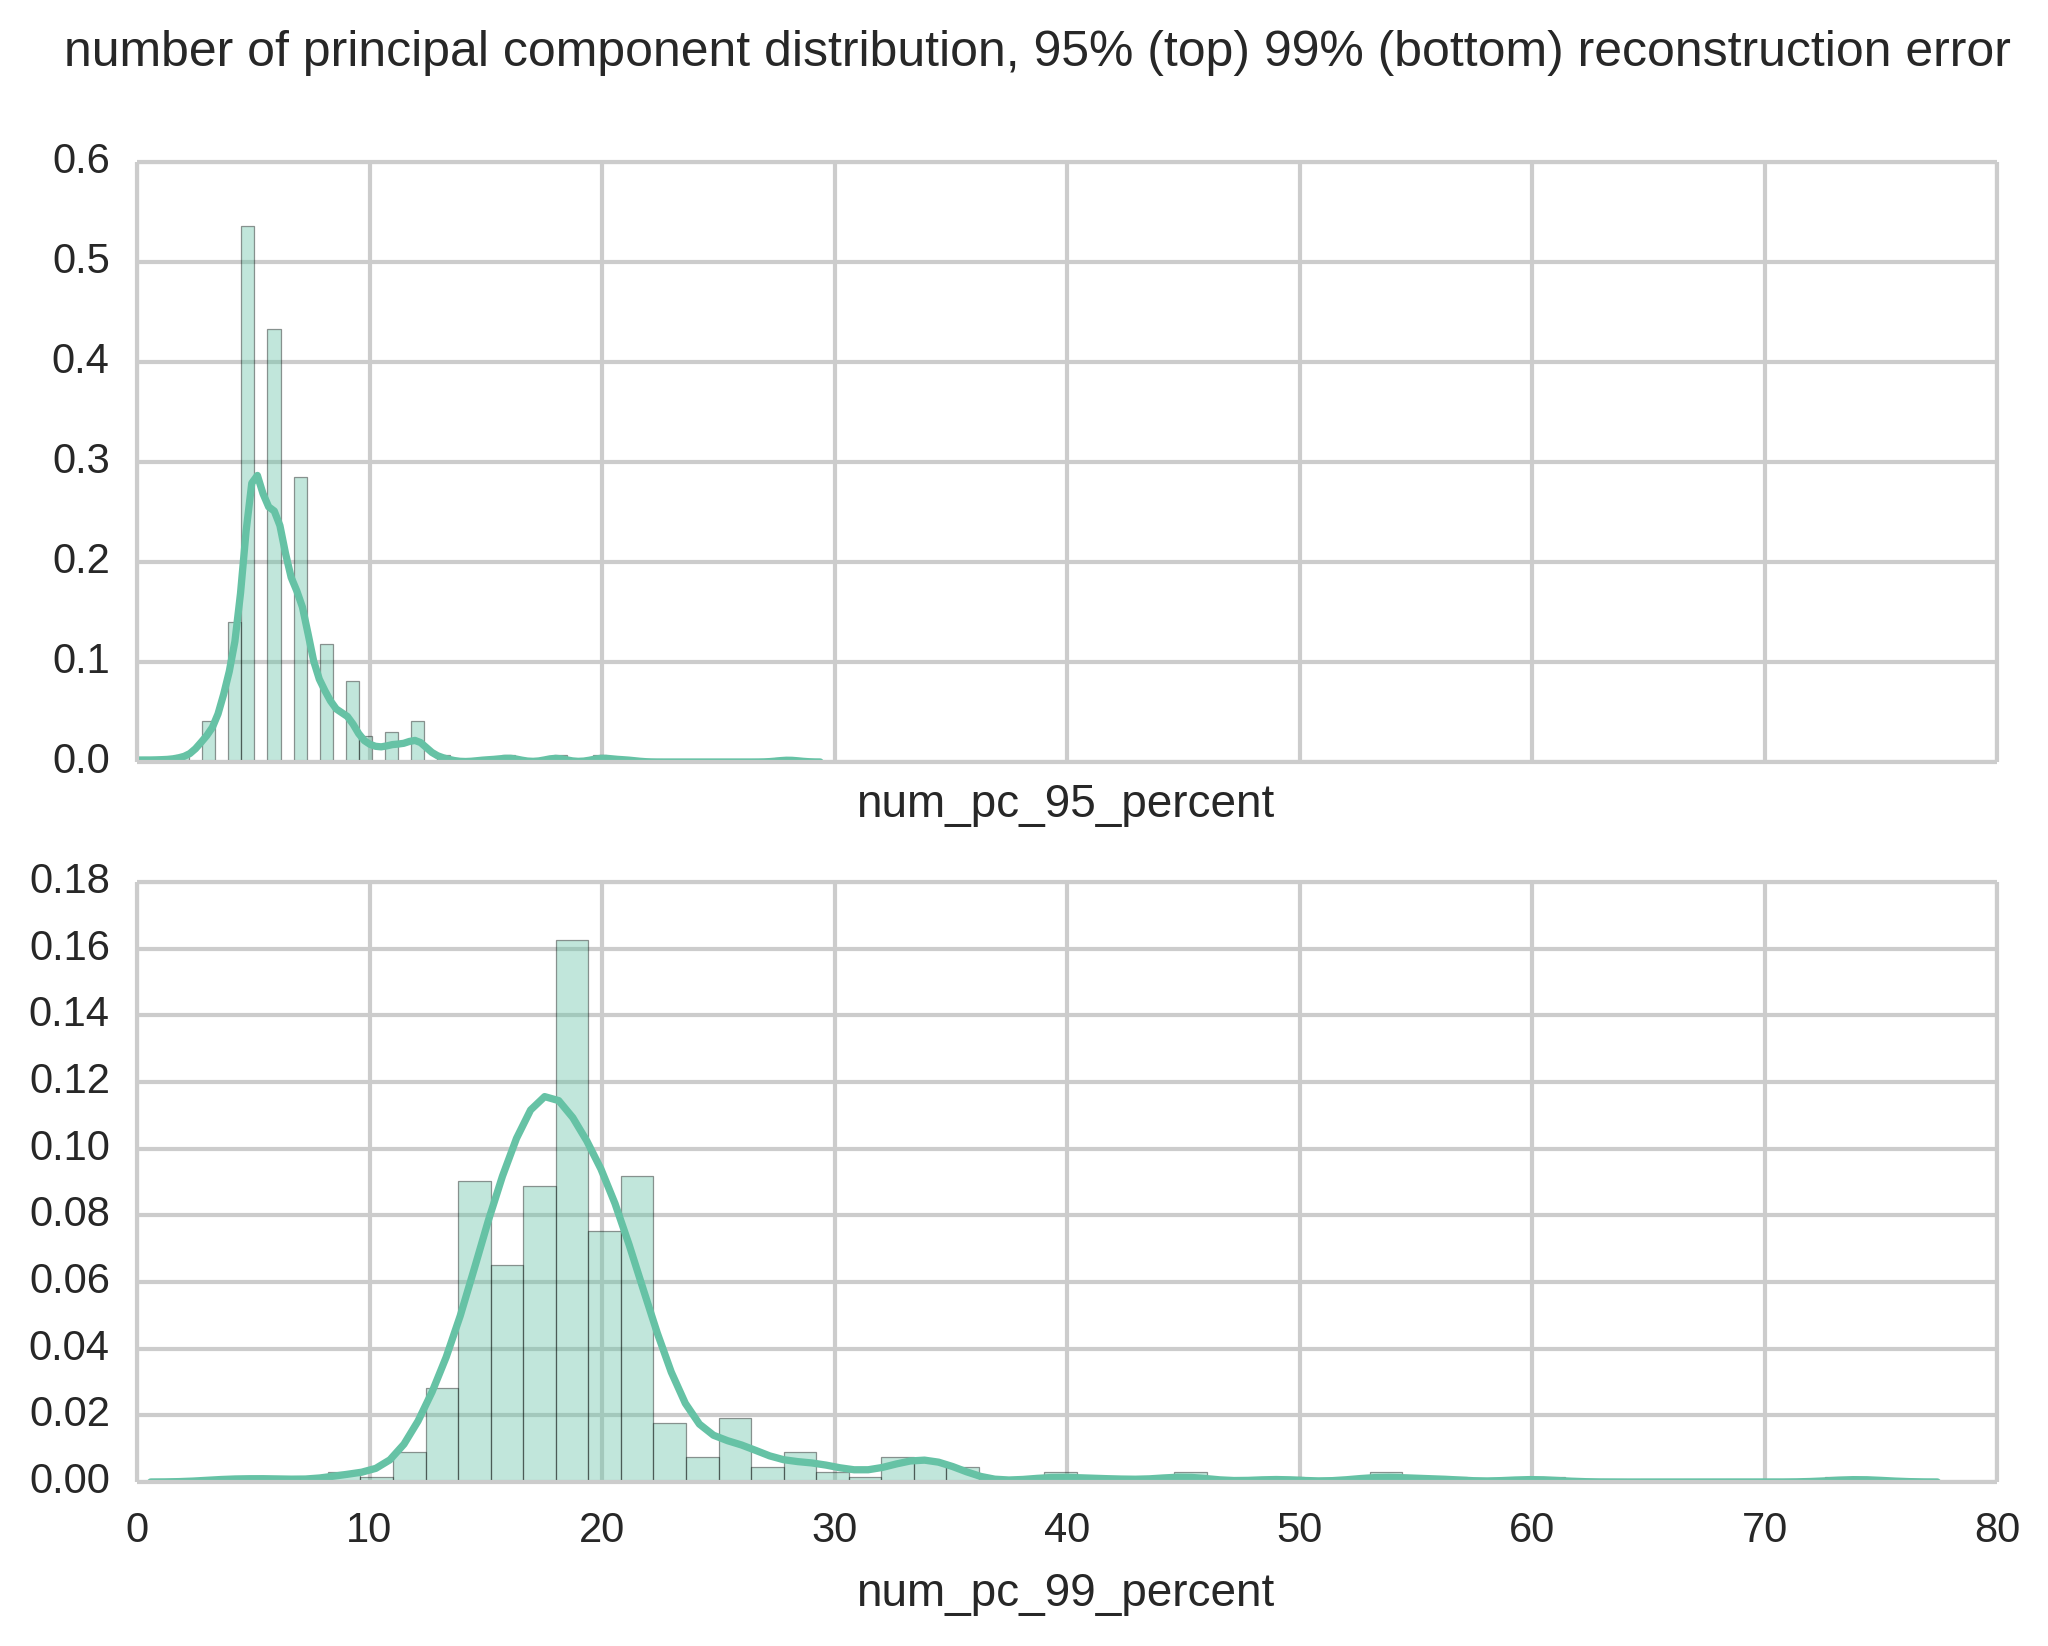
\includegraphics[width=0.8\textwidth]{images/num_pcs.png}
  \caption{Number of principal components with 95 and 99 percent reconstruction error}
  \label{fig:num_pcs}
\end{figure}
\FloatBarrier
\small
\begin{verbatim}
Accounted for 95% variance
n_pc  n_building
5     145
6     117
7      77
4      38
8      32
9      22
3      11
...

Accounted for 99% variance
n_pc  n_building
18    64
17    60
20    51
19    46
15    45
16    44
21    35
...
\end{verbatim}

Weather station and number of PCs
\begin{verbatim}
ICAO	num_pc_95_percent	num_pc_99_percent
---------------------------------------------------
KLCH	8	                22
KDDH	6	                19
KPLN	7	                20
KCXY	5	                17
...
\end{verbatim}
For the experiment building ``OR0033PE'', a plot of the number of pcs and the varience accounted for are shown in \fref{fig:pcs}
\begin{figure}[h!]
  \centering
  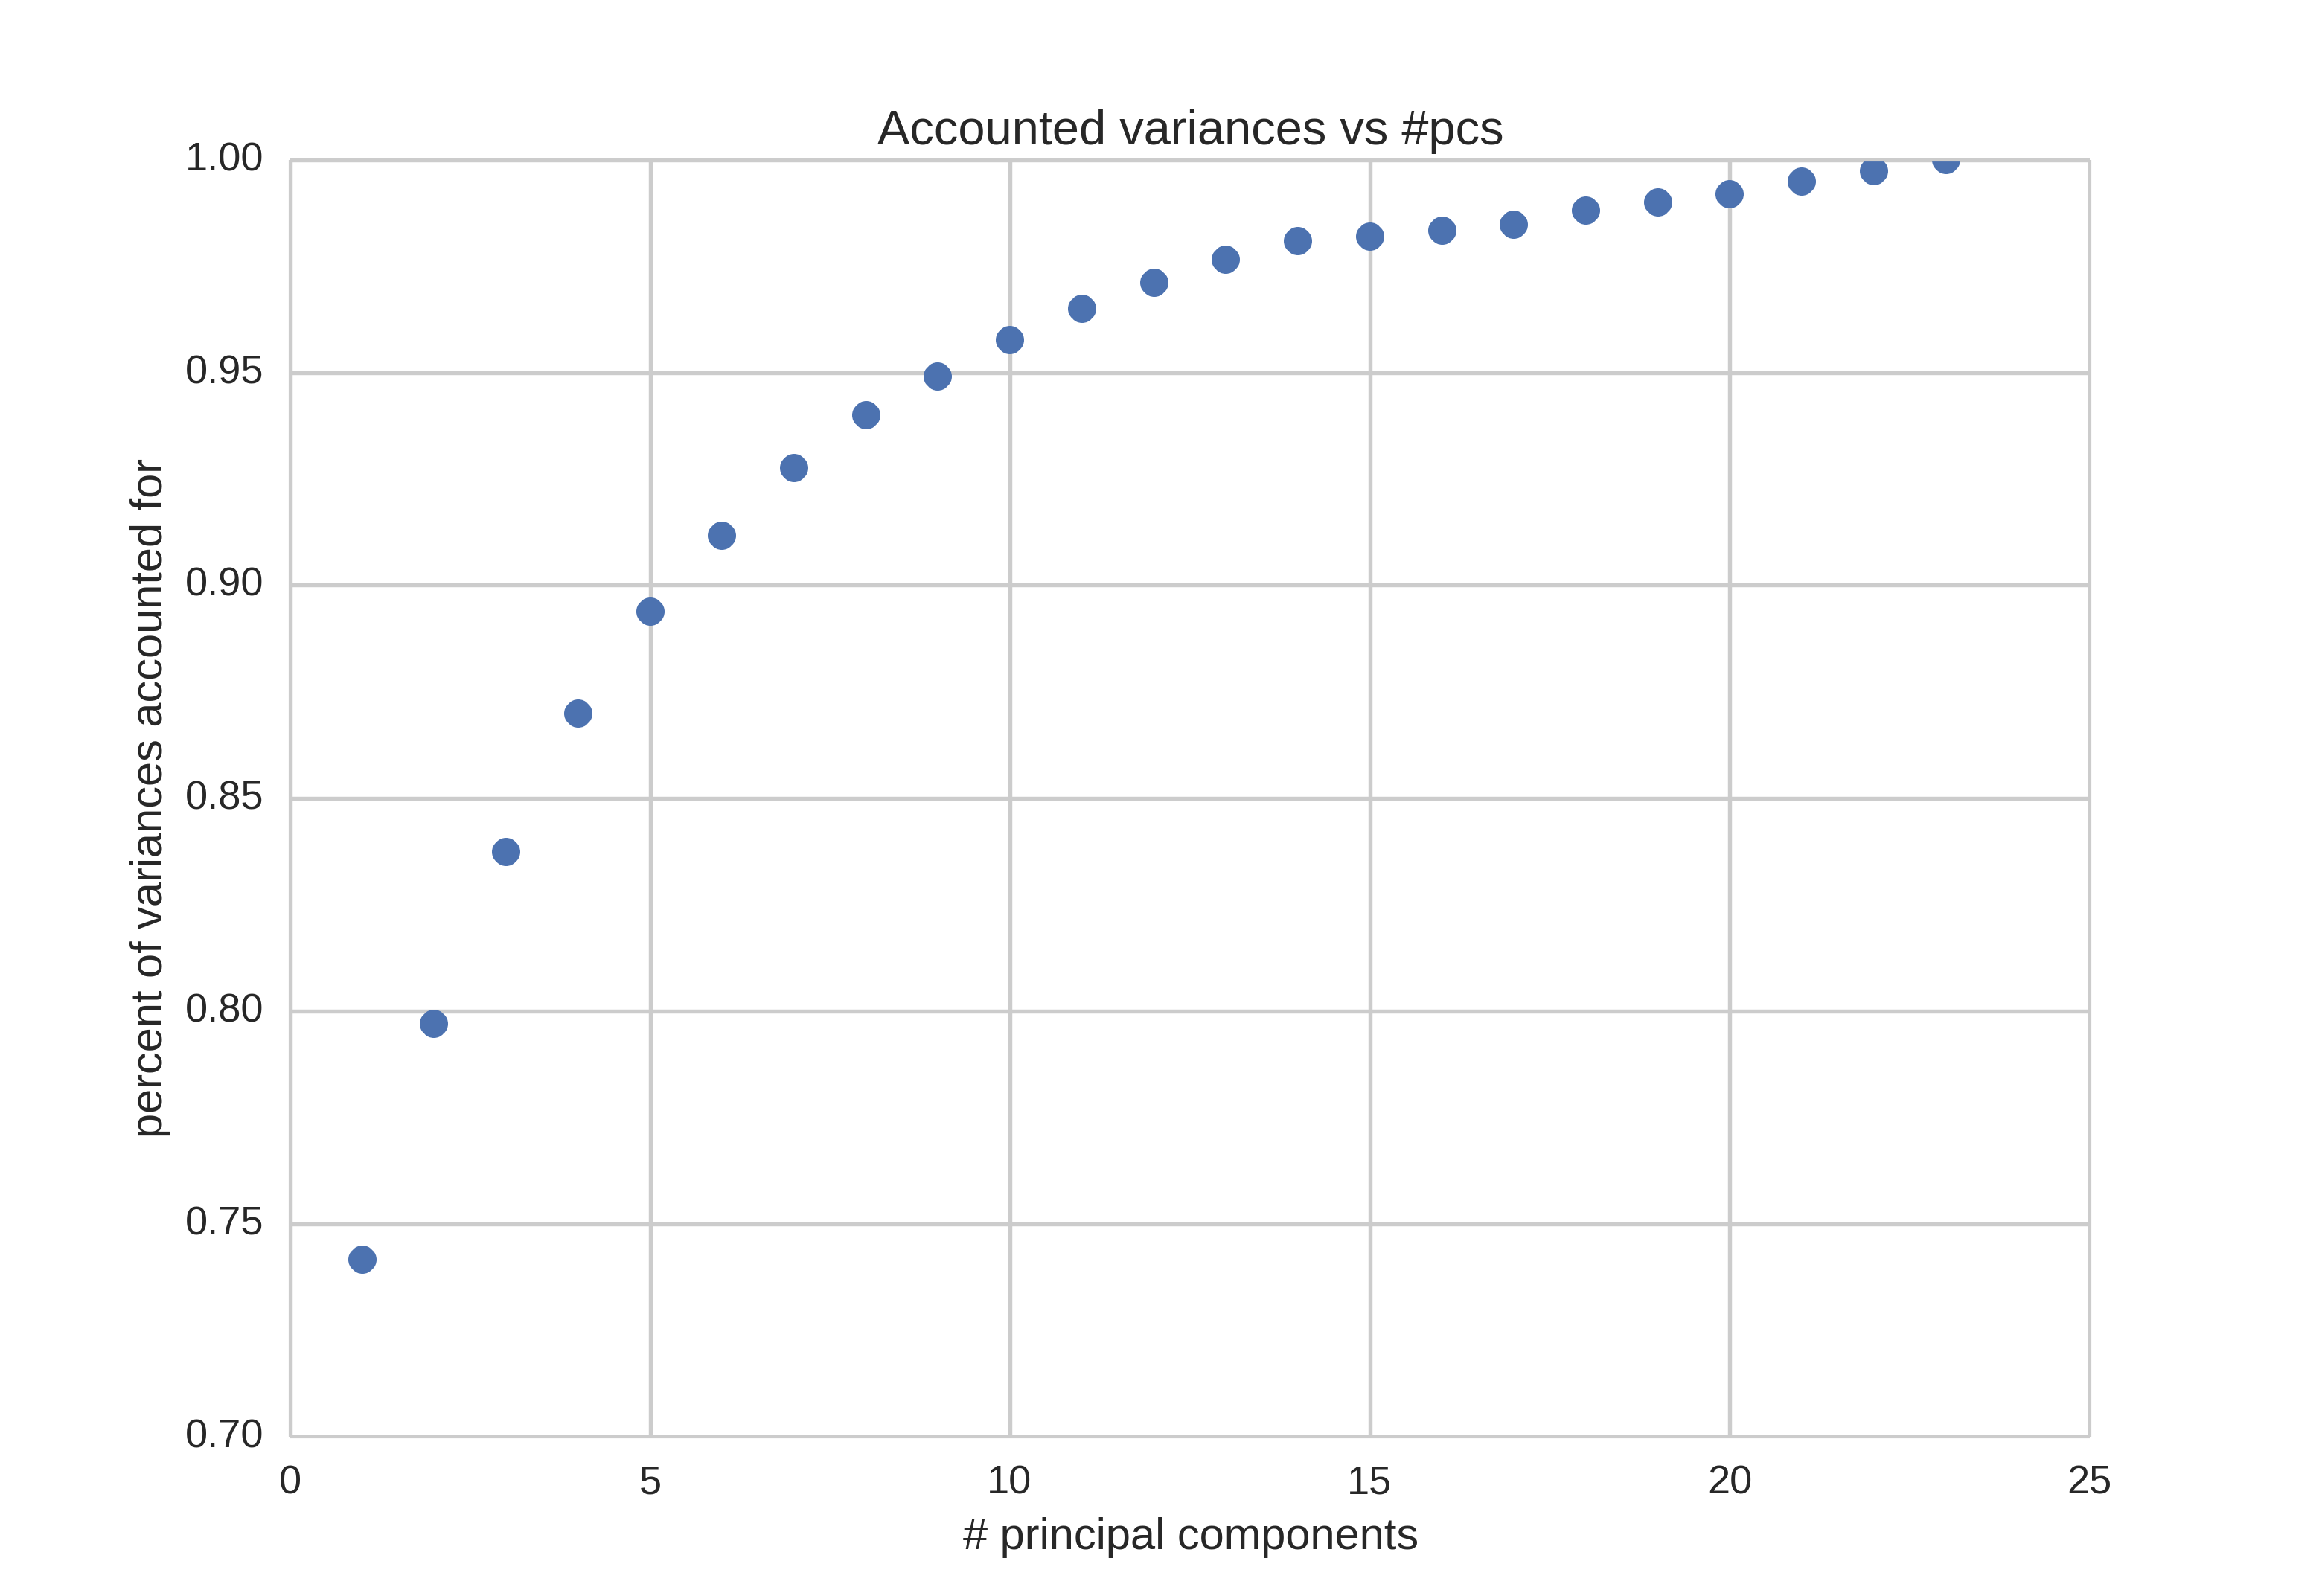
\includegraphics[width=0.6\textwidth]{images/pca_err_numpc_OR0033PE.png}
  \caption{Accounted variance and the number of pcs}
  \label{fig:pcs}
\end{figure}

\subsection{Use PCs as independent variables for the regression}
For the test building ``OR0033PE'', using 1 to 10 PCs with ordinary least square linear regression, the error achieved are (note: this part is implemented using Python \texttt{sklearn.decomposition.PCA}, the ``accounted variance'' is different from the previous session when using \texttt{linalg.eig})
\begin{verbatim}
num_PC accounted variance mse
1      0.765992063661     16.5442958987
2      0.81918354379      17.5088737364
3      0.852882590053     17.5473191338
4      0.879556033684     17.668850597
5      0.899650396008     17.9211677598
6      0.916688494142     17.9019603561
7      0.932492047507     18.0952033615
8      0.942872262315     18.1477157171
9      0.952484921675     18.1519075386
\end{verbatim}
The smallest prediction error is when only using the first principal
component (\fref{fig:pca_err_pc}), but it is still dramatically larger
than the other methods.
\begin{figure}[h]
  \centering
  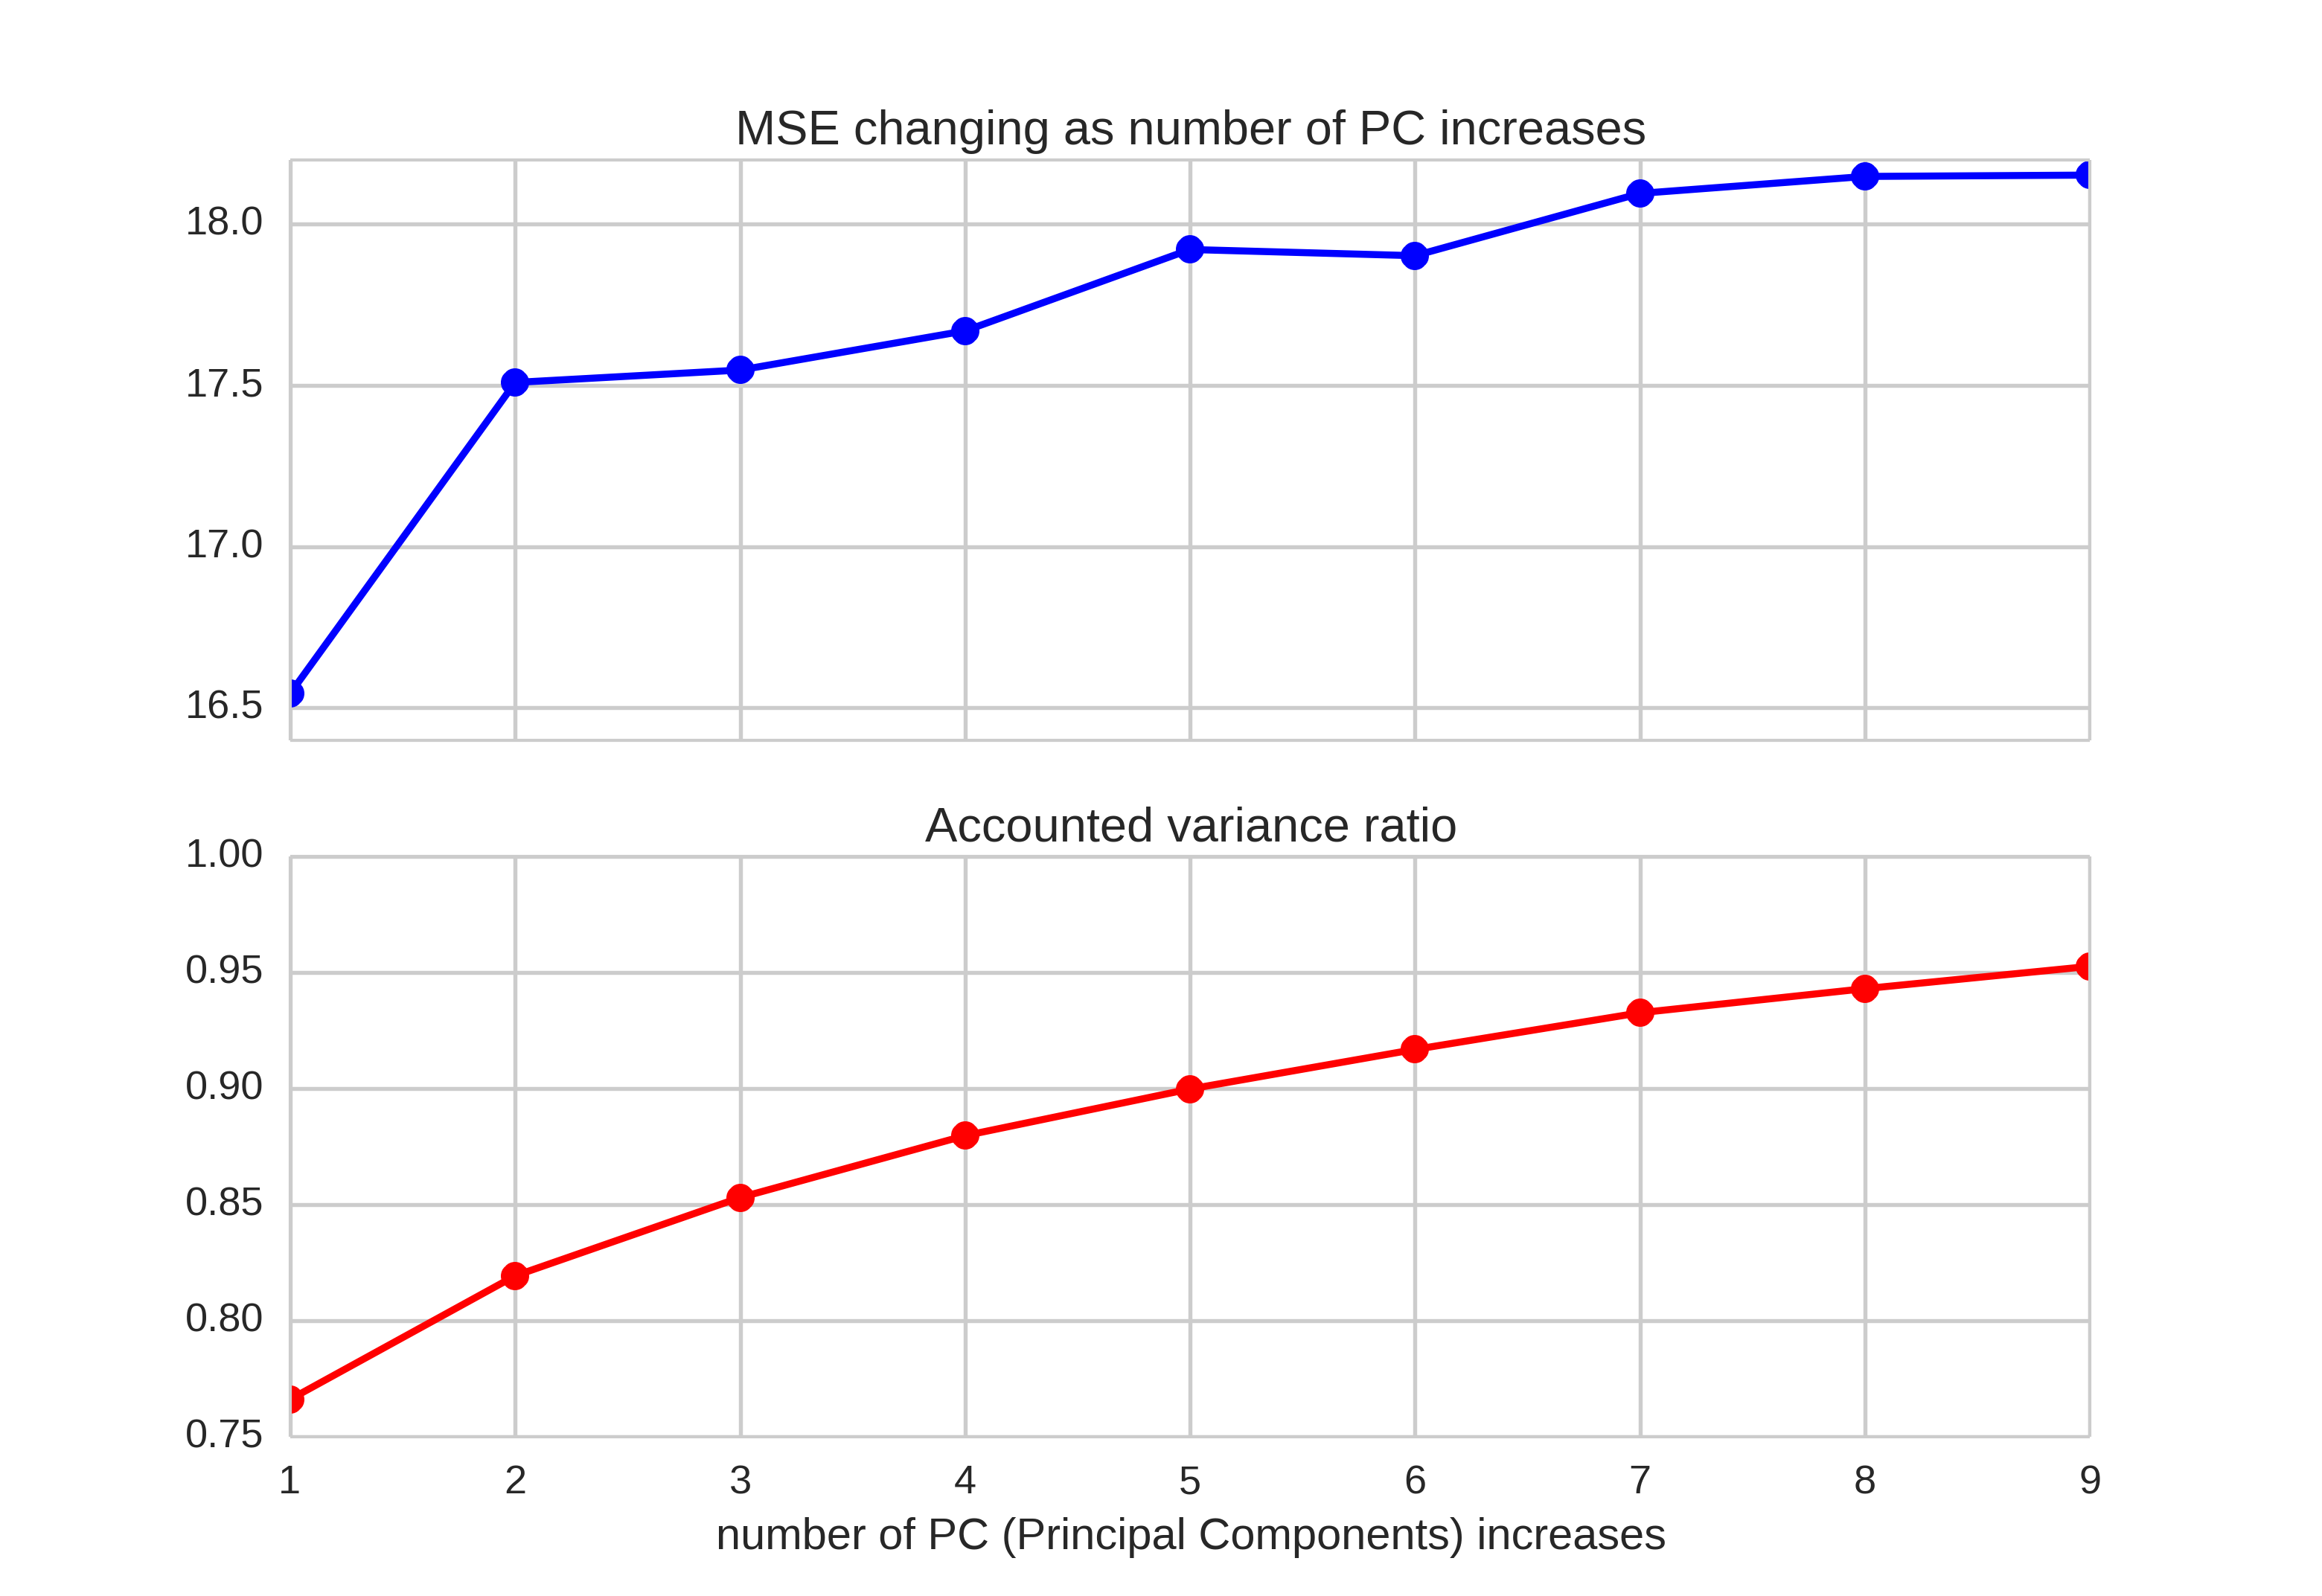
\includegraphics[width=0.8\textwidth]{images/pca_err_pc.png}
  \caption{Error vs number of principal components}
  \label{fig:pca_err_pc}
\end{figure}
\FloatBarrier

\subsection{Proposed method 3: Auto-encoder with non-linear activation function}
An auto-encoder contains an encoding function $\phi$, and a decoding
function $\psi$. It minimizes the re-construction error:
$\left\|X - \psi(\phi)X\right\|^2$
% bookmark

To be implemented...

\subsection{Proposed method 4: Fused lasso with degree day base 40F to 80F}
Fused lasso is ``a generalization that is designed for problems with
features that can be ordered in some meaningful
way''~\cite{tibshirani2005sparsity}, penalizing the difference of
adjacent coefficients.

\begin{comment}
\section{Summary result}
\begin{table}[h!]
  \centering
  \begin{tabular}{c|c}
    \hline
    model&MSE\\
    \hline
    \hline
    piecewise linear&2.07631642389\\
    ridge regression&1.37049790455\\
    PCA&16.5442958987\\
    auto encoding& to be implemented...\\
    \hline
  \end{tabular}
  \caption{result of testing the methods above on building ``OR0033PE''}
  \label{tab:summaryResult}
\end{table}
\FloatBarrier
\section{next stage}
\subsection{Problem specification}
\begin{itemize}
\item using a set of features to predict hourly energy
\item using a set of features to predict monthly energy we know the duration of the energy record
\item using a set of features to predict hourly energy we do not know the duration of the energy record
\end{itemize}
\subsection{Broad idea}
From the discussing with Professor
~\href{http://www.cs.cmu.edu/~mgormley/}{Matt Gormley}, the broad
approach should be: first create a rich feature set with all
potentially related features included, and use a non-linear model on
the rich feature set so that the training data can be nearly perfectly
predicted. Then applying some regularization to also drive down the
test error. Finally try to interpret the model by evaluating the
accuracy drop by leaving each feature out, or by incrementally adding
a feature in random order and evaluate the accuracy gain by adding
that feature.
\subsection{Collect input variables and representation}
A list of features to be included in the next stage model are
\begin{itemize}
\item Environmental variable
  \begin{itemize}
  \item outdoor air temperature: exact hourly temperature, Radio Basis
    Function Kernel (RBFs), or temperature with exponential smoothing
  \item Humidity
    \begin{itemize}
    \item relative humidity (RH) as exact measurement or as with exponential smoothing
    \item dew point temperature
    \end{itemize}
  \item solar radiation ($W / m^2$)
  \item Wind speed (scaler)
  \end{itemize}
\item Occupancy
  \begin{itemize}
  \item Operation schedules
  \item Occupancy ratio (ratio of occupied vs non-occupied days)
  \end{itemize}
\item Building type
\item Time
  \begin{itemize}
  \item weekday vs weedend
  \item hour of day
  \item day of week
  \item time lag ($k$), the number of previous readings to include in the model
  \item unit circle representation of time of day, week, month, and year
  \end{itemize}
\item Energy
  \begin{itemize}
  \item power ($W$, it's an auto-regressive component: use energy to
    predict energy) of previous $k$ time steps.
  \item fuel type: Electric vs non-electric
  \end{itemize}
\item Floor area
\item pre-retrofit and post-retrofit period
\end{itemize}

\section{Data sources}
\begin{itemize}
\item \href{https://www.wunderground.com/}{weather underground}: Time (EST), Temp., Windchill, Dew,Point,
  Humidity, Pressure, Visibility, Wind,Dir, Wind,Speed, Gust,Speed,
  Precip, Events, Conditions
\begin{verbatim}

\end{verbatim}
\end{itemize}
\subsection{Non-linear models}
\begin{itemize}
\item Neuron Network with 1-2 hidden layer
\item Support Vector Regression with RBF kernel
\item Random forest regression~\cite{randomForestWiki2016}
\item piecewise linear regression as baseline (it's a simple non-linear model, but not expressive enough)
\end{itemize}

\newpage
\bibliographystyle{plain}
\bibliography{myCitation}
\end{document}